\begin{figure}[h]
        \centering
        \begin{subfigure}{.49\textwidth}
          \centering
          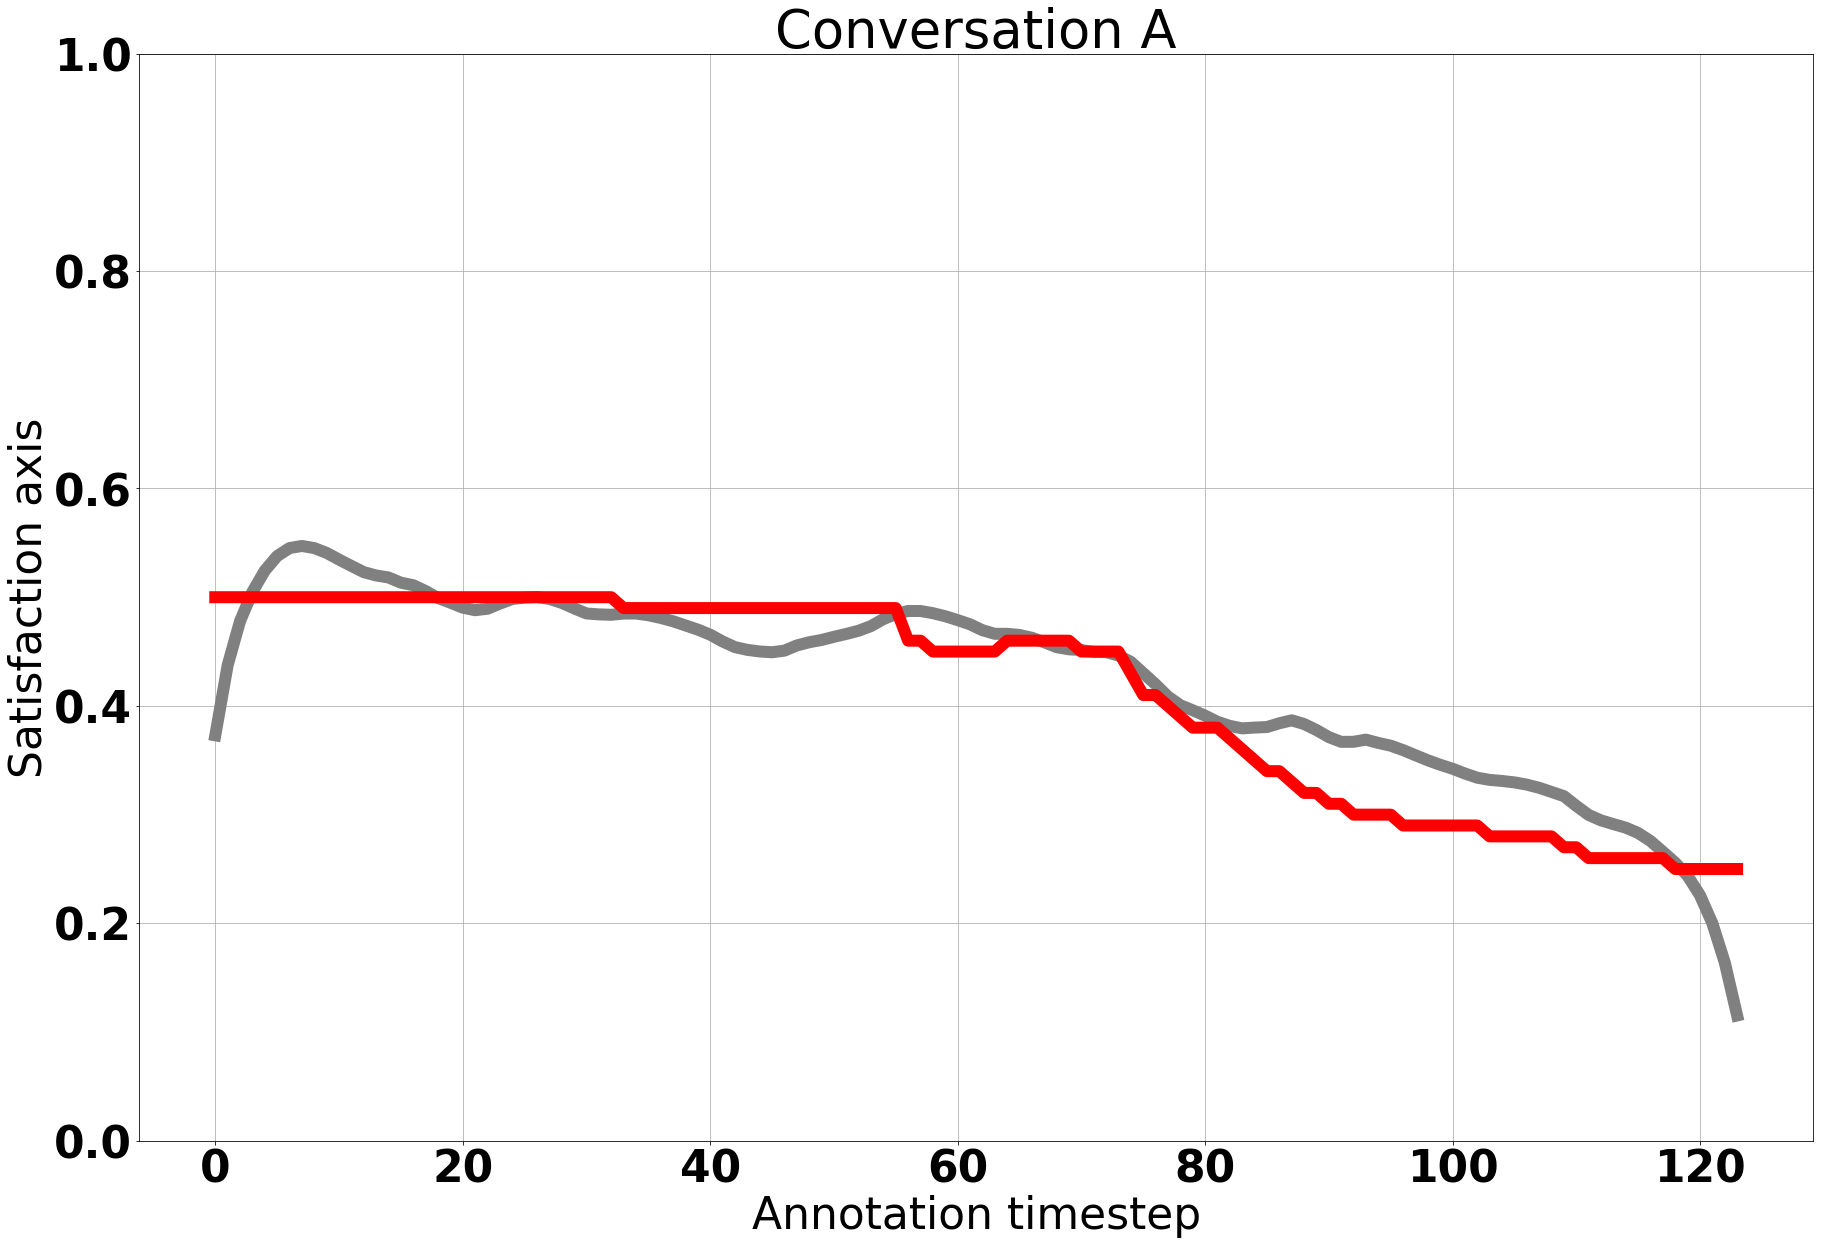
\includegraphics[width=.99\linewidth]{./Chapitre5/figures/cccVSrmse1.png}
        \end{subfigure}
        \begin{subfigure}{.49\textwidth}
          \centering
          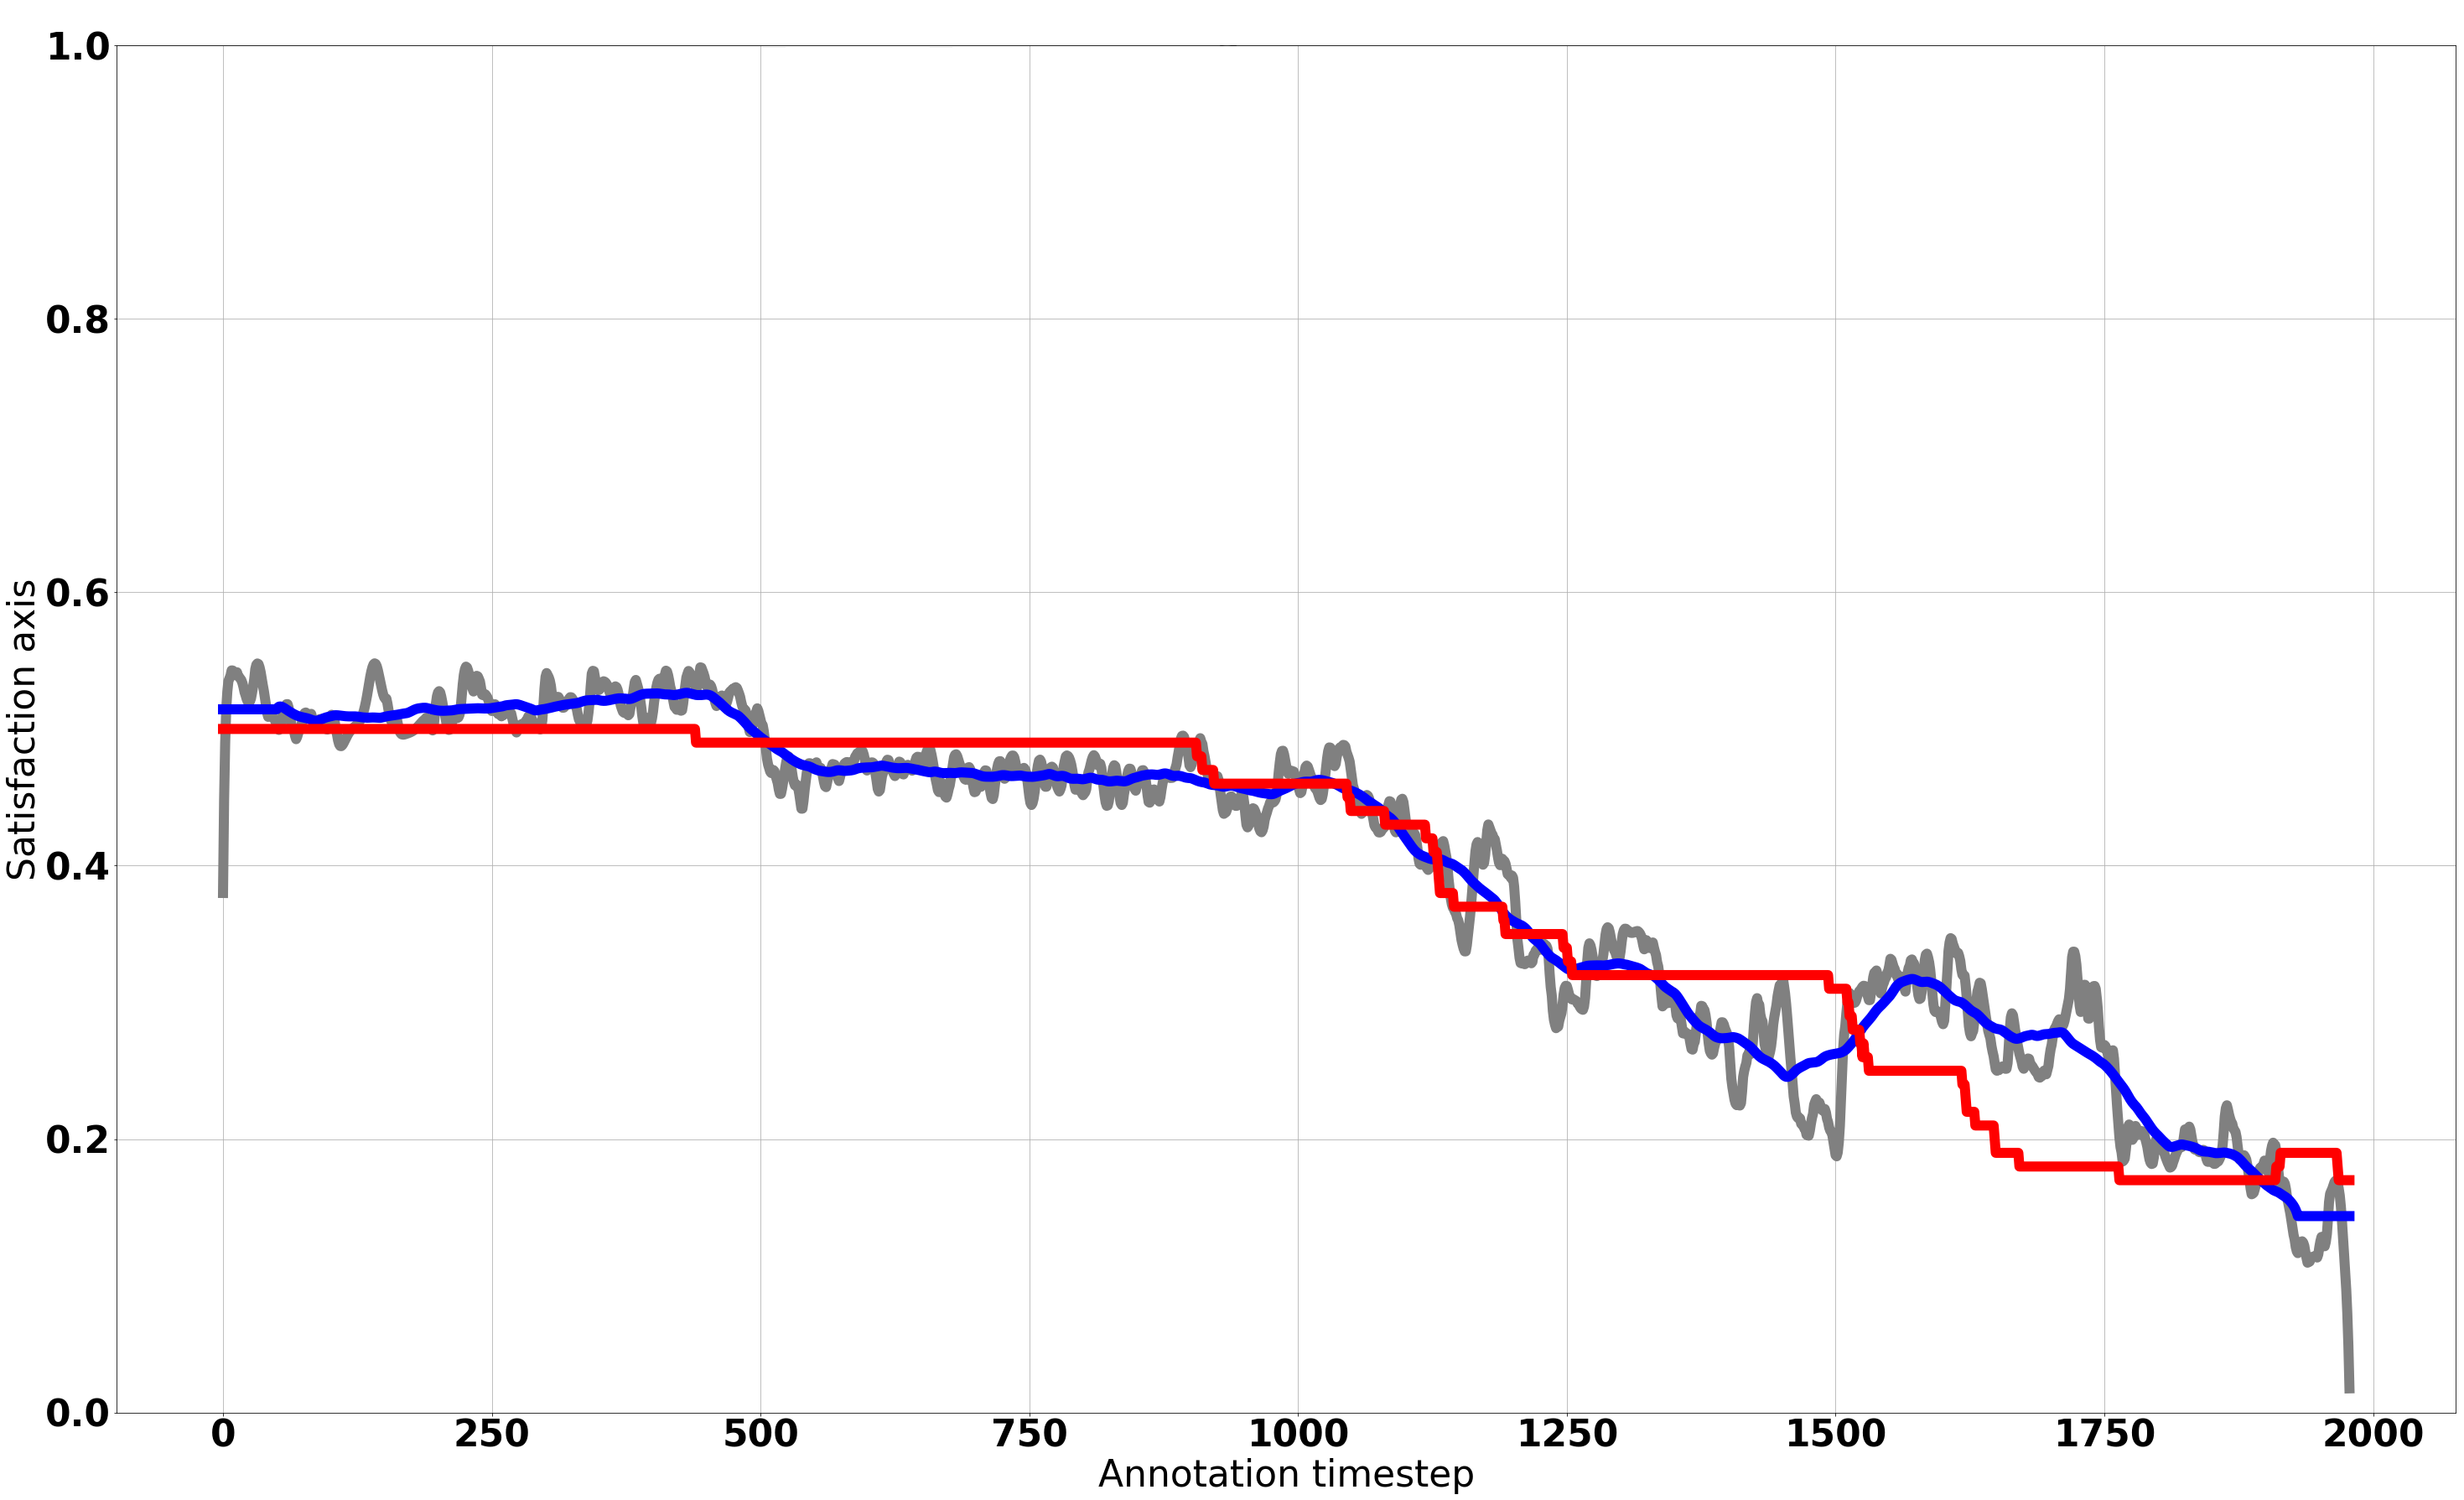
\includegraphics[width=.99\linewidth]{./Chapitre5/figures/lissage2.png}
        \end{subfigure}
        \caption{Evolution des prédictions (grises) et des références (rouge) de deux conversations provenant de l'ensemble de test d'AlloSat. $ccc(A) = 0.564$, $ccc(B) = 0.903$. La courbe bleue correspond au lissage des prédictions. Obtenu avec le système biLSTM-4 (l-rmse) et Mfcc-lib.}
        \label{fig:cccVSrmse}
    \end{figure}
